\documentclass[11pt]{article}

\usepackage[utf8]{inputenc}
\usepackage{enumerate}
\usepackage{amssymb}
\usepackage{amsfonts}
\usepackage{amsthm}
\usepackage{graphicx}
\usepackage[ruled,vlined]{algorithm2e}

% New commands
\newcommand{\xt}{$(X_t)$ }
\newcommand{\om}{$\Omega$ }
\renewcommand\qedsymbol{$\blacksquare$}

% New Environment
\newtheorem{theorem}{Theorem}
\newtheorem{conjecture}{Conjecture}
\newtheorem{propriete}{Property}[subsection]
\newtheorem{proposition}{Proposition}[subsection]
\newtheorem{corollary}{Corollary}[subsection]
\newtheorem{definition}{Definition}[subsection]
\newtheorem{lemma}{Lemma}[subsection]
\newtheorem{remarque}{Remark}[subsection]

% Numbering equations


\begin{document}

\title{Lattice polytopes random sampling using Markov chains}
\author{Julien David, Lionel Pournin, Rakotonarivo Rado}
\maketitle

\noindent{\textbf{Abstract.}} This paper describes an approach of random sampling of lattice polytopes contained in a $[0,k]^d$ hypercube, denoted by $(d,k)-$polytopes. This method consists in modeling a Markov chain where the space of states $\Omega$ is the set of polytopes of dimension $d$ contained in the $[0,k]^d$ hypercube coupled with a set of several transition rules. Given $d$ and $k$, we run a random walk on the chain until we reach a stationnary distribution. We prove that such a chain is irreducible, aperiodic and has the uniform as stationnary distribution, hence a uniform random sampler of $(d,k)-$polytopes. We also give an upper bound for the mixing time for $d = 2$.

\section{Introduction}

A Markov chain is a process wich evolves in time on a space of states $\Omega$. It is characterized by its transition matrix $P$, which describes the transitions between the states of $\Omega$.

It is a common way to model a Markov chain in order to sample random objects, then run a random walk on it until one reaches a stationnary distribution. Under some conditions one can ensure an uniform distribution on the space of state $\Omega$. In this paper, this process will be used to build a random sampler for the lattice polytopes contained in the $[0,k]^d$ hypercube. From now such polytope will be denoted as $(d,k)-$polytope.

This paper will be structured as follows. First a reminder on the essential results on Markov chains we used in our proof will be given. Then, the concrete Markov chain we modeled will be discribed. Finally we will give a proof to our main results on the chain.

\section{Reminders on Markov chains}

Let us beging on some reminders on some important propreties already known on Markov chains. Since the number of lattice polytopes contained in the $[0,k]^d$ is finite, we only take into account Markov chains with a finite space of state.

\subsection{Definitions}

A \textit{Markov chain} $(X_t)_{t\geq{0}}$ with a finite space of state $\Omega$ is a process evolving in time on the elements of $\Omega$. Moving from an element $x \in \Omega$ to another state follows a fixed distribution $P(x,\cdot)$. $(X_t)_{t\geq{0}}$ is a sequence of random variables $(X_0, X_1, \cdots)$ which has its values in $\Omega$. The \textbf{Markov property} on $(X_t)$ ensures that at the value of the chain at time $t+1$  only depends of the value of the chain at the time $t$.

The \textit{transition matrix} $P$ of $(X_t)$ defines the transition between the states of $\Omega$. $P$ is stochastic and its $x-$th row refers to the distribution $P(x,\cdot)$. One has:

\begin{equation}
  \sum_{y \in \Omega} P(x,y) = 1 \quad \forall{x \in \Omega}
\end{equation}

The \textit{graph} $\mathcal{G}(V,E)$ of $(X_t)$ is the graph where the vertices are the states of $\Omega$. There is an edge between two vertices $x$ and $y$ of the graph if there exits a transition form $x$ to $y$ on $(X_t)$, that is $P(x,y)=1$.

\begin{figure}
  \begin{center}
    \includegraphics[width=5cm]{assets/frog}
    \caption{A Markov chain such that: $\Omega = \{x,y\}$, $P(x,x) = 1-p$, $P(x,y) = p$,  $P(y,x) = q$ and $P(y,y) = 1-q$}
    \label{fig:fig1}
  \end{center}
\end{figure}



\subsection{Properties}

Let $(X_t)_{t\geq{0}}$ be a Markov chain, $\Omega$ its space of state and $P$ its transition matrix. This section will focus on the propreties of a Markov chain we are interested in.


\begin{propriete}
  The transition matrix $P$ of $(X_t)$ is \textbf{irreducible} if there exists a $r_0$ such that for all $x$ and $y \in \Omega$, $P^r(x,y)$ when $r>r_0$.
\end{propriete}

This means that every single state of $\Omega$ can be reached from any other state. Then, we define by $\mathcal{T}(x)=\{t\geq{1} \ : P^t(x,x)>0\}$ the set of the times when the chain gets back at the state $x\in \Omega$. The \textbf{period} of $x$ is defined by $\mathrm{gcd}(\mathcal{T}(x))$.

\begin{propriete}
  $(X_t)$ is \textbf{aperiodic} if all states in $\Omega$ has a period $1$, otherwise it is called \textbf{periodic}.
\end{propriete}

\begin{propriete}\label{prop:irr-ap}
  If $P$ is irreducible then all the state of $\Omega$ has the same period.
\end{propriete}

\begin{propriete}
  $(X_t)$ is said to be \textbf{symetric} if for all $x$ and $y$ in $\Omega$, one has the same probability to move from $x$ to $y$ and from $y$ to $x$, i.e: $P(x,y) = P(y,x)$ for all $x,y \in \Omega$.
\end{propriete}

% HITTING TIME, FIRST RETURN TIME, RECURRENCE OF A STATE

% For all state $x \in \Omega$, we define the \textbf{hitting time} by $\tau_x=\min \{t\geq{0} \ : X_t = x\}$. It is the time when time the chain visits $x$ for first time. For situations where only a visit to $x$ at positive time will do, we define $\tau_x^+=\min \{t\geq{1} \ : X_t = x\}$. If $X_0 = x$, $\tau_x^+$ is called \textbf{first return time}.

% A state $x$ is \textbf{positive recurrent} if $\mathrm{E}_x(\tau_x^+)<\infty$, where $\mathrm{E}_x(\tau_x^+)$ is the expectation of the first return time at $x$ starting from $x$. This simply means that this quantity represents the average of time spent between two consecutive visits on $x$.

\subsection{Stationnary distribution and mixing time}

We note by $\mu_t$ the row vector giving the probability distribution on $\Omega$ at the time $t$, and by $\mu_t(x)$ the probability to be at $x$ at the time $t$, this means that $\mu_t(x) = \mathbf{P}\{X_t = x \} \quad \forall x \in \Omega$. In order to obtain the distribution $\mu_{t+}$, one has to apply one time to $\mu_t$ the transition matrix $P$, on the right. That is:

\begin{equation}
  \mu_t = \mu_{t-1}P \quad \forall t\geq{1}
\end{equation}

Starting from an initial distribution $\mu_0$, one has $\mu_t = \mu_0P^t \quad \forall t\geq{0}$. In particular, a distribution is called \textbf{stationnary} if it satisfies:

\begin{equation}
  \pi = \pi P
\end{equation}

In another words, one has:

\begin{equation}
  \pi(y) = \sum_{x \in \Omega} \pi(x)P(x,y) \quad \forall y \in \Omega
\end{equation}

The stationnary distribution $\pi$ can be viewed as the average amont of time spent by the chain at each state of $\Omega$.

For a chain $(X_t)$, the \textbf{mixing time} is the smallest time needed until we reach a stationnary distribution if it exists. In our case, we are willing to reach an uniform distribution over $\Omega$. The mixing time will determine the efficiency of our sampler.

\begin{propriete}\label{prop:irr_ap}
  If $P$ is irreducible and aperiodic, there exists $\pi$, a distribution over $\Omega$ such that $\pi = \pi P$ and $\pi(x)>0$ for all $x$ in $\Omega$. Furthermore if $(X_t)$ is symetric, then the uniform distribution over $\Omega$ is a stationnary distribution of $(X_t)$.
\end{propriete}

% \begin{propriete}\label{prop:uniqueness}
%   An irreducible chain with a finite space of state is positive recurrent, meaning that all its states are positive recurrent. It has an unique stationnary distribution $\pi$.
% \end{propriete}

\section{$(d,k)-$polytopes model}

Let us recall that we aim to build an uniform random sampler of $(d,k)-$polytopes. This section will describe our Markov chain model in order to do so. Given $d$ and $k$, let us consider the $[0,k]^d$ hypercube. The main idea of the sampler is to run random walk on a Markov chain $(X_t)$ which space of state $\Omega$ is the set of $(d,k)-$polytopes. The transition matrix $P$ will be described as a set of local rules on our $(d,k)-$polytopes.

A $d$ dimension \textbf{polytope} $\mathcal{P}$ is a convex hull of a finite set of points $\mathcal{A}$ in a $d$ dimension euclidian space . The points of $\mathcal{A}$ which consist the convex hull are called the \textbf{vertices} of $\mathcal{P}$. A polytope is called a \textbf{lattice polytope} if all its vertices have integer values. We call a $d$ dimension \textbf{simplex} a polytope with $d+1$ vertices.

In our case we define a point $v$ as an \textbf{interior point} of $\mathcal{P}$ if $v$ is either inside or on the boundary of $\mathcal{P}$ and $v$ is not a vertex of $\mathcal{P}$.

\subsection{Notations and context}

First let us set the context of the sampler. The objects we will to sample are the $(d,k)-$polytopes. Then let the space of state $\Omega$ of $(X_t)$ be the set of $(d,k)-$polytopes, given $d$ and $k$.

A \textbf{state} $x$ is a set of $l$ points in $[0,k]^d$ which form a convex hull with exactly $l$ vertices, i.e. $x=\{v_1, v_2, …, v_l\}$ where all the $v_i\in[0,k]^d$ for all $i \in [1,l]$. The the number of vertices of $x$ will be called its size and noted by $|x|$. Since $x$ is a set of point but as well a convex hull, we will assume that $x=\{v_1, v_2, …, v_l\}$ means $x=Conv(\{v_1, v_2, …, v_l\})$.

\begin{enumerate}
  \item $x-\{v_j\}$ is the convex hull in which we had remove exactly the $j-$th vertex of $x$. We note that $x-\{v_j\}$ is also a state of $\Omega$, and it is fulldimentional only if $|x|>d+1$.
  \item $x \cup \{v\}$ where $v \in [0,k]^d$, is the convex hull where we add exactly one point without removing any of the $l$ vertices of $x$. We can observe that $|Conv(x \cup \{v\})| = |x| + 1$.
\end{enumerate}

\subsubsection{Transition rules}

The \textbf{transition rules} over $\Omega$ is defined as local operations on our $(d,k)-$polytopes. Actually our set of rules consists in either adding or removing one vertex to move up from one state to another. Let $x$ and $y$ be two states in $\Omega$. We draw uniformally a point $v \in [0,k]^d$, then consider the following rules:

\begin{itemize}
  \item If $v$ is an interior point of $x$ then we loop on $x$, meaning the chain stays on $x$.
  \item If $v$ is a vertex of $x$ then:
  \begin{itemize}
    \item If $x$ is not a simplex, remove $v$ from $x$ and we have a transition from $x$ to $y=x - \{v\}$. We have this transition only when $x$ is not a simplex since $y$ is fulldimentional only if $|x|>d+1$.
    \item If $x$ is a simplex, we loop on $x$.
  \end{itemize}
  \item If $v$ is drawn outside $x$ then compute the convex hull of $x \cup \{v\}$:
  \begin{itemize}
    \item If $Conv(x\cup\{v\})$ is exactly $x\cup\{v\}$, means $|Conv(x \cup \{v\})| = |x| + 1$, then we have a transition from $x$ to $y = x \cup \{v\}$.
    \item Else we loop on $x$.
  \end{itemize}
\end{itemize}

% \begin{figure}
%   \begin{center}
%     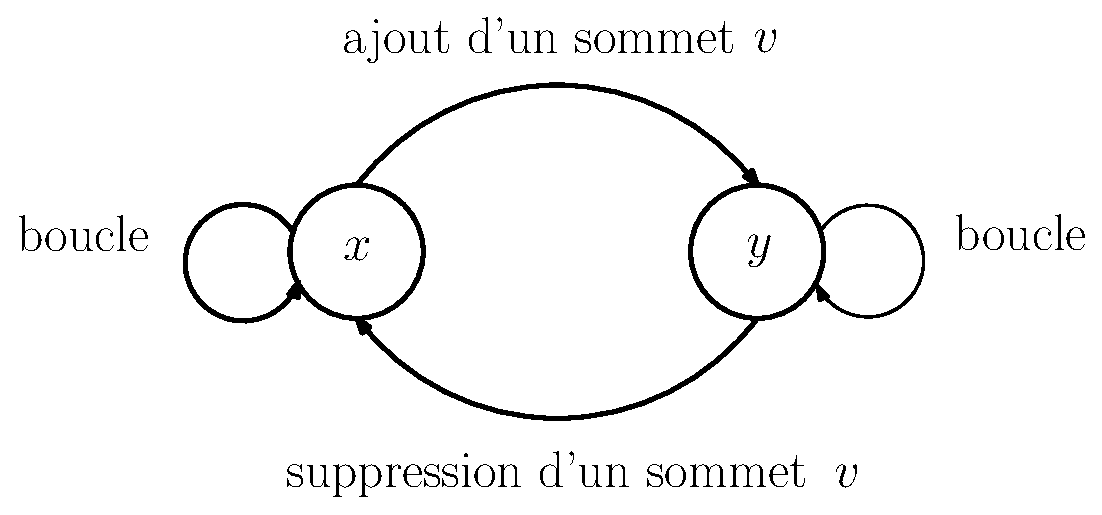
\includegraphics[scale=0.3]{assets/transition}
%     \caption{Transition relation between two states $x$ and $y$ in $\Omega$: either $y = x \cup \{v\}$ and $x = y - \{v\}$ or $v$ has been moved respectivly from $x$ to get $y/$ from $y$ to get $x$, where $v \in [0,k]^d$.}
%     \label{fig:fig2}
%   \end{center}
% \end{figure}

\begin{figure}
  \begin{center}
    \includegraphics[scale=0.9]{assets/boucle}
    \caption{For $[0,4]^2$. Cases where we stay on $x$: (1) $v$ is an interior point of $x$, $P(x,x) = 1$. (2) $v$ is a vertex of $x$, we stay on $x$. (3) $v$ is drawn outside $Conv(x)$ but $|Conv(x\cup\{v\})| \neq |x|+1$, $P(x,y) = 0$. }
    \label{fig:boucle}
  \end{center}
\end{figure}

\section{Properties of $(X_t)$}

Let us now consider $(X_t)$ as defined above. This section will verify properties on $(X_t)$, which are mainly the irreducibility, the symetry and the periodicity. Before doing so, it is important to introduce the symetric difference notion which will be used for our proof.

\subsection{Symetric difference}

Given $x$ and $y \in \Omega$, we define their \textbf{symetric difference} $x \bigtriangleup y$ such that:

\begin{equation}
  x \bigtriangleup y = \{ u \in x : u \notin y \ \mbox{et} \ v \in y : v \notin x \}
\end{equation}

% Here the symetric difference applied on two polytopes can be viewed in the same way as in the set theory, $x \bigtriangleup y = x \cup y \setminus x \cap y$, nevertheless some remarks worth mentioning:
%
% \begin{itemize}
%   \item $x \cup y$ is not always a convex hull.
%   \item $x \bigtriangleup y = x \setminus y \cup y \setminus x$
%   \item $|x \cup y| = |x| + |y|$ if $x \cap y = \emptyset$.
%   \item $x \bigtriangleup y$ is maximal when $x$ and $y$ do not have any common vertices.
% \end{itemize}

Introducing the symetric difference will help us in the proof of the irreducibility of $(X_t)$. In fact move from $x$ to $y$ in our chain consists in finding finite number of transitions between $x$ and $y$. Observe that the simplest way to move from $x$ to $y$ consists in adding directly to $x$ the vertices of $y$ then remove $x$ vertices. This means that at each step one reduces the symetric difference between $x$ and $y$. Hence, one can verify that the cardinality of $x \bigtriangleup y$ is a lower bound for the distance, noted $\delta(x,y)$, between $x$ and $y$. One has: $\delta(x,y) \geq{|x \bigtriangleup y|}$.

However, we might face cases which not allow this fast transition, thus we have to find out other transition state instead of those \textit{trivial} cases.

\begin{lemma}\label{lem:elim-mauvais-cas}
  For any simplex $x \in \Omega$, for any $y \in \Omega$. If we cannot reduce $x \bigtriangleup y$ by adding a vertex in $y \setminus x$ the there exists a simplex $z \in \Omega$, a transition state between $x$ and $y$, which verifies:
  \begin{itemize}
    \item $|x \bigtriangleup y| = |z \bigtriangleup y|$
    \item $\delta(x,z)\leq{2}$
  \end{itemize}
  such that we can always add a vertex in $y \setminus z$, from $z$ to $y$.
\end{lemma}

\begin{proof}
  Lionel.
\end{proof}

\begin{lemma}\label{lem:irreducibility}
  For all $x$ and $y \in \Omega$, there exists $z \in \Omega$ which satisfies $|x \bigtriangleup y| > |z \bigtriangleup y|$ such that $\delta(x,z)\leq{3}$.
\end{lemma}

\begin{proof}
  Let $x$ and $y$ be states of $\Omega$, such that $P(x,y)=0$. Let $z$ be a transition state between $x$ and $y$, and such that $z$ is closer to $y$ than $y$. We have several distinct cases:

  \begin{enumerate}
    \item $x$ is not a simplex.
    \begin{enumerate}
      \item $x \subset y$: add $v \in y \setminus x$ and $z = x \cup \{v\}$, then $\delta(x,z) = 1$
      \item $x \not\subset y$: remove $v \in x \setminus y$ and $z = x - \{v\}$, then $\delta(x,z) = 1$
    \end{enumerate}
    \item $x$ is a simplex.
    \begin{enumerate}
      \item If we can add $v \in y \setminus x$ then add it, thus $z = x \cup \{v\}$ and $\delta(x,z) = 1$
      \item Else:
      \begin{enumerate}
        \item Add a point $u$ which is not in $x \bigtriangleup y$
        \item Remove a point from  $x \setminus y$
        \item Add  a point from $y \setminus x$

        In this last case, one finds $z$ such that $\delta(x,z) = 3$
      \end{enumerate}
    \end{enumerate}
  \end{enumerate}

  Since we had proved we can always add a point which is not contained in $x \bigtriangleup y$ by lemma \ref{lem:elim-mauvais-cas}. It means that wherever in which case we are, one can always find a $z$ which reduces the symetric difference from $z$ to $y$ by one, such that $\delta(x,z) \leq{3}$.

\end{proof}

\begin{corollary}\label{coro:diameter}
  For all $x$ and $y \in \Omega$ one has:
  \begin{equation}
    \delta(x,y) \leq |x| + |y| + 4(d+1)
  \end{equation}
\end{corollary}

\begin{proof}
  This is an immediate consequence of the lemma \ref{lem:irreducibility}. Let $x$ and $y$ be in $\Omega$. Let us now consider two simplices $x^\star$ and $y^\star$ such that $\delta(x,x^\star) = |x| - (d+1)$, and $\delta(y,y^\star) = |y| - (d+1)$. Then $\delta(x,y) \leq{\delta(x,x^\star) + \delta(x^\star,y^\star) + \delta(y,y^\star)}$.
  Since $x^\star$ is a simplex, the walk needs at most $3(|x^\star| + |y^\star|) = 3 \times 2(d+1)$ steps to reach $y^\star$ from $x^\star$. Hence $  \delta(x,y) \leq{|x| - (d+1) + |y| - (d+1) + 6(d+1)} = |x| + |y| + 4(d+1)$.
\end{proof}

Observe that corollary \ref{coro:diameter} gives an idea on the upper bound of the diameter of $(X_t)$. We have now settled all we need to prove our main results on the properties of $(X_t)$.

\begin{theorem}\label{thm:diameter}
  Define the diameter $\mathcal{D}$ of a graph with vertex set $\Omega$ to be the maximum distance between two vertices. For $(X_t)$, as defined above, and given $k$ and $d$, one has:
  \begin{equation}
    \mathcal{D}_{X_t} \leq{2ck^{3/4} + 4(d+1)} \quad \mbox{where} \ c>0
  \end{equation}
\end{theorem}

\begin{proof}
  To be done.
\end{proof}

\begin{theorem}\label{thm:main}
  The Markov chain $(X_t)$ is irreductible, aperiodic and has the uniform as stationnary distribution.
\end{theorem}

\begin{proof}
  Three propreties have to be verified, thus this proof will be given in three steps. Let $x$ and $y$ be in $\Omega$.

  \begin{enumerate}[i]
    \item \textit{Irreducibility}
    Irreducibility is a direct consequence of the corollary \ref{coro:diameter}. Let us remind that to prove the irreducibility, one needs to find a $r_0$ such that, for all $x$ and $y \in \Omega$, when $r \geq{r_0}$ then $P^r(x,y)>0$. Thus let us take $r_0 = |x| + |y| + 4(d+1)$.

     \item \textit{Symetry}
     Our transition rules consists in either add or remove a single vertex for two distinct states. Observe that if there is no one step transition from $x$ to $y$ means $P(x,y)=0$. By the trasition rules, necessarily, if $P(x,y)=0$ then $P(y,x)=0$.
     Next, let us prove that if $P(x,y)>0$ and $P(y,x)>0$ then we also have $P(x,y) = P(y,x)$. $P(x,y)>0$ means that we have a one step transition from $x$ to $y$. Only two cases may occur. For $v \in [0,k^d]$ either $y = x - \{v\}$, or $y = x \cup \{v\}$. Considering the first case, the probability to draw $v$ and add it to $x$ is $P(x,y) = \frac{1}{(k+1)^d}$. Similarily, to move from $y$ to $x$, we draw the same $v$ and remove it from $y$ to get $x$ with probability $P(y,x) = \frac{1}{(k+1)^d} = P(x,y)$. We prove the remaining case in an analog reasoning.

     \item \textit{Aperiodicity}

     To prove that $(X_t)$ is aperiodic, one needs to show that each state in $\Omega$ has as period $1$. Since $(X_t)$ is irreductible, property \ref{prop:irr-ap} tells us that all the states of $\Omega$ has the same period. Thus, for all $x, y \in \Omega$, $\mathrm{gcd}(\mathcal{T}(x)) = \mathrm{gcd}(\mathcal{T}(y))$. One needs to find a state $x$ such that t$\mathrm{gcd}(\mathcal{T}(x)) = 1$. Let us take $x$ has a simplex and a point $v \in [0,k]^d$ then consider the cases where we have a loop on $x$:
     either $v$ is an interior point to $x$, or $v$ is drawn outside of $x$ but $|Conv(x \cup \{v\})| \neq |x| + 1$. One has: $P(x,x) = \mathbf{P}\{v \  \mbox{interior point to} \ x\} + \mathbf{P}\{v \in x\} + \mathbf{P}\{|x \cup \{v\}| \neq |x| + 1\}$.
     Note that $\mathbf{P}\{v \in x\} = \frac{1}{(k+1)^d}$, but since $|x| = d+1$, we have a loop on $x$ with probability $P(x,x) \geq{\frac{1}{(k+1)^d}} > 0$. In another words, with positive probability the walk can get back to $x$ from $x$ in one step. Hence, $\mathcal{T}(x) = \{1, \dots\}$. We conclude that $\mathrm{gcd}(\mathcal{T}(x)) = 1$.

   \end{enumerate}
\end{proof}

\section{Random sampler}

Consider $(X_t)$ as defined previously. Sampling random $(d, k)$-polytopes consists in a random walk on $\Omega$ with our transition rules until one reaches the stationnary distribution. The amount of time needed to reach such a distribution, that is sample a uniformally random $(d, k)$-polytope, is the mixing time on $(X_t)$.

Sampling a random $(d, k)$-polytope with this model is given the following algorithm.

\vspace{0.5cm}

\begin{algorithm}[H]\label{Algo.RS}
  \LinesNumbered
  \DontPrintSemicolon
  \KwIn{the dimension $d$, the size $k$ of the hypercube}
  \KwOut{a random lattice $(d,k)$-polytope}
  \BlankLine

  sample a random lattice $(d,k)$-simplex $P$ with vertex set $\mathcal{V}$\;
  \While{we are not close enough to the stationary distribution}{
  generate a random lattice point $x$ in $[0,k]^d$\;
  \If{$x \in \mathcal{V}$ and $\mathrm{conv}(\mathcal{V}\mathord{\setminus}\{x\})$ is $d$-dimensional}{
    $P \leftarrow \mathrm{conv}(\mathcal{V}\mathord{\setminus}\{x\})$\;
   }
  %\Else{$|\mathrm{conv}(\mathcal{V} \cup \{x\})|$ == $|\mathcal{V}| + 1$}{
  \Else{
    compute the convex hull $Q$ of $\mathcal{V}\cup\{x\}$\;
    \If{the vertex set of $Q$ is $\mathcal{V}\cup\{x\}$}{
      $P \leftarrow \mathrm{conv}(\mathcal{V} \cup \{ x\})$\;
    }
  }
 }
 \Return{$P$}
 \caption{Random sampling of a lattice $(d, k)$-polytope}
\end{algorithm}


\begin{theorem}\label{thm:random-sampler}
  The random sampler $\Gamma(d,k)$ described by algorithm \ref{algo1} is a uniform random sampler of $(d,k)-$polytopes over $\Omega$.
\end{theorem}

\section{Results on mixing time}



\clearpage
\bibliographystyle{plain}
\bibliography{biblio.bib}

\end{document}
